\documentclass[a4paper]{article}
\usepackage{float}
\usepackage[utf8]{inputenc}
\usepackage[T1]{fontenc}
\usepackage{graphicx}
\usepackage[frenchb]{babel}
\usepackage{amsmath}
\usepackage{listings}
\usepackage{hyperref}

% define our color
\usepackage{xcolor}

% code color
\definecolor{ligthyellow}{RGB}{250,247,220}
\definecolor{darkblue}{RGB}{5,10,85}
\definecolor{ligthblue}{RGB}{1,147,128}
\definecolor{darkgreen}{RGB}{8,120,51}
\definecolor{darkred}{RGB}{160,0,0}

% other color
\definecolor{ivi}{RGB}{141,107,185}


\lstset{
    language=scilab,
    captionpos=b,
    extendedchars=true,
    frame=lines,
    numbers=left,
    numberstyle=\tiny,
    numbersep=5pt,
    keepspaces=true,
    breaklines=true,
    showspaces=false,
    showstringspaces=false,
    breakatwhitespace=false,
    stepnumber=1,
    showtabs=false,
    tabsize=3,
    basicstyle=\small\ttfamily,
    backgroundcolor=\color{ligthyellow},
    keywordstyle=\color{ligthblue},
    morekeywords={include, printf, uchar},
    identifierstyle=\color{darkblue},
    commentstyle=\color{darkgreen},
    stringstyle=\color{darkred},
}

\begin{document}

\title{VISA -- TP Segmentation}
\author{Arnaud Cojez}
\date{mercredi 16 novembre 2016}

\maketitle

\newpage
\tableofcontents
\newpage
%----------------------------------------------------------------------------------------
%	INTRODUCTION
%----------------------------------------------------------------------------------------

\section{Introduction}

Nous avons vu dans le précédent TP comment étaient représentées les couleurs en informatique. Dans ce TP, nous allons tenter de segmenter des images par classification de pixels.\\

Nous devrons écrire une Macro ImageJ qui permet de segmenter une image en un nombre donné de classes. Nous segmenterons ensuite d'autres images en utilisant ces classes et observerons les résultats, à la fois dans les espaces RGB et HSB.

\begin{figure}[H]
\begin{center}
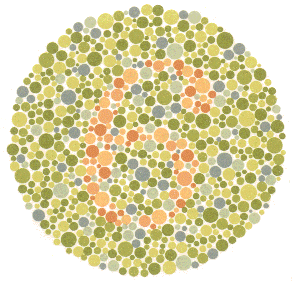
\includegraphics[width=170px]{../base/cas_4_dalton6.png}
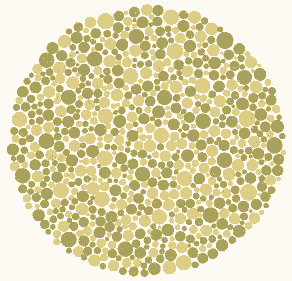
\includegraphics[width=170px]{../resultats/cas_4_dalton6_seg.png}
\end{center}
\end{figure}

\begin{figure}[H]
\begin{center}
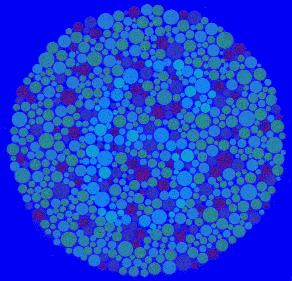
\includegraphics[width=170px]{../resultats/cas_4_dalton6_hsb.png}
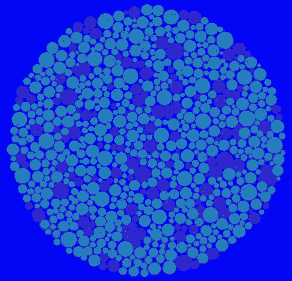
\includegraphics[width=170px]{../resultats/cas_4_dalton6_hsb_seg.png}
\end{center}
\end{figure}

\clearpage
%----------------------------------------------------------------------------------------
%	SEGMENTATION DES IMAGES
%----------------------------------------------------------------------------------------
\section{Segmentation des images par K-Means et discrimination linéaire}

\subsection{Explication}
Le but ici est d'écrire une macro qui permet dans un premier temps de segmenter une image en un nombre donné de classes.
Pour ce faire nous utilisons l'algorithme supervisé K-Means grâce au plugin Segmentation > K-Means Clustering fourni.\\

Nous parcourons ensuite l'image Cluster Centroid Values afin de stocker les valeurs RGB des différentes classes.\\

Puis nous demandons à l'utilisateur d'ouvrir une nouvelle image.\\

Ensuite, nous segmentons la nouvelle image en sélectionnant pour chaque pixel la classe dont la couleur est la plus proche de la couleur courante (dans l'espace RGB).

{\em La Macro a été fournie en pièce jointe.}

\subsection{Résultats}

\subsubsection{Segmentation par K-means}

Nous testons dans un premier temps la macro sur l'image {\em cas\_3\_dalton15}, en demandant 3 classes. Nous obtenons l'image segmentée ci-dessous (à droite) ainsi que les valeurs des différentes classes.

\begin{figure}[H]
\begin{center}
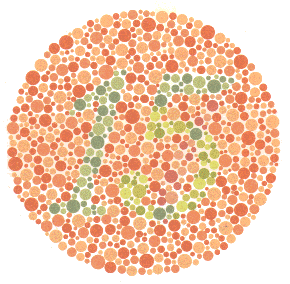
\includegraphics[width=170px]{../base/cas_3_dalton15.png}
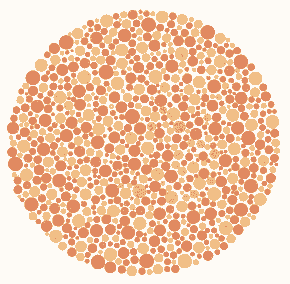
\includegraphics[width=170px]{../resultats/cas_3_dalton15_seg.png}
\end{center}
\caption{À gauche : Image initiale | À droite : Image segmentée}
\end{figure}

\clearpage
\subsubsection{Classes obtenues}

Après analyse de l'image, nous retrouvons les 3 classes de couleurs suivantes :

\begin{enumerate}
  \item R=254, G=251, B=246
  \item R=241, G=191, B=135
  \item R=225, G=138, B=97
\end{enumerate}

\subsubsection{Segmentation par distance euclidienne}

Nous devons maintenant ouvrir une nouvelle image. Nous sélectionnons {\em cas\_3\_dalton74} pour la segmenter selon la méthode citée plus haut. Voici le résultat obtenu.

\begin{figure}[H]
\begin{center}
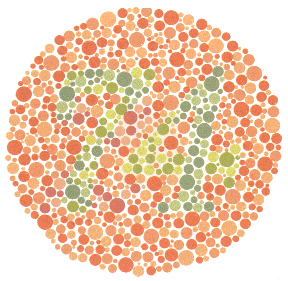
\includegraphics[width=170px]{../base/cas_3_dalton74.png}
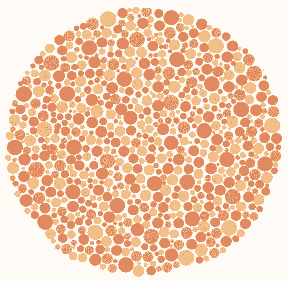
\includegraphics[width=170px]{../resultats/cas_3_dalton74_seg.png}
\end{center}
\caption{À gauche : Image initiale | À droite : Image segmentée}
\end{figure}

\clearpage
%----------------------------------------------------------------------------------------
%	APPLICATION
%----------------------------------------------------------------------------------------
\section{Application aux images {\em cas\_4}}

\subsection{Explication}

Le but de cette partie est d'appliquer la macro codée dans la partie précédente et d'observer les résultats sur le lot d'images {\em cas\_4}, à la fois dans l'espace RGB et HSB.\\

La première image sélectionnée et segmentée est l'image {\em cas\_4\_dalton6}. Nous utiliserons les 3 classes extraites de cette image afin de segmenter les images suivantes.

\subsection{Résultats}

\subsubsection{Image {\em cas\_4\_dalton6} dans l'espace RGB}

Après classification et segmentation par la méthode K-Means, nous obtenons l'image ci-dessous (à droite).

\begin{figure}[H]
\begin{center}
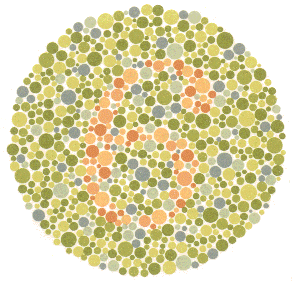
\includegraphics[width=170px]{../base/cas_4_dalton6.png}
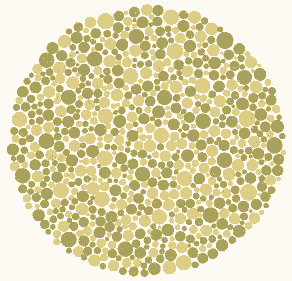
\includegraphics[width=170px]{../resultats/cas_4_dalton6_seg.png}
\end{center}
\caption{À gauche : Image initiale | À droite : Image segmentée}
\end{figure}

Les classes obtenues sont les suivantes :

\begin{enumerate}
  \item R=252, G=250, B=242
  \item R=222, G=206, B=133
  \item R=168, G=162, B= 93
\end{enumerate}

Nous voyons que les points de couleurs sont pour la plupart bien segmentés, mais nous ne pouvons pas distinguer les chiffres présents initialement.\\
Nous allons donc tester cet algorithme dans l'espace HSB afin de voir si la segmentation nous donne des résultats plus utiles.

\clearpage
\subsubsection{Image {\em cas\_4\_dalton6} dans l'espace HSB}

Nous analysons les résultats de cette macro dans l'espace HSB.\\
Ainsi, nous convertissons l'image choisie dans l'espace HSB, nous obtenons l'image ci-dessous à gauche, puis nous utilisons la même méthode que dans la partie précédente. Nous obtenons l'image ci-dessous à droite.

\begin{figure}[H]
\begin{center}
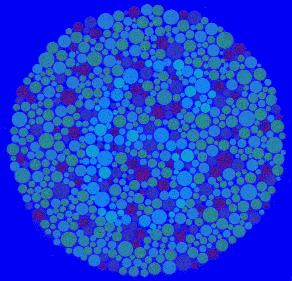
\includegraphics[width=170px]{../resultats/cas_4_dalton6_hsb.png}
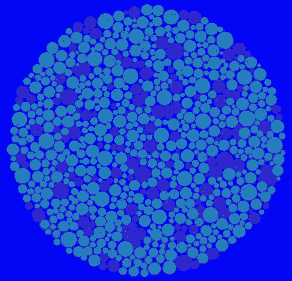
\includegraphics[width=170px]{../resultats/cas_4_dalton6_hsb_seg.png}
\end{center}
\caption{À gauche : Image initiale (HSB) | À droite : Image segmentée}
\end{figure}

Les classes obtenues sont les suivantes :

\begin{enumerate}
  \item R=  3, G=  5, B=245
  \item R= 46, G= 39, B=205
  \item R= 36, G=125, B=188

\end{enumerate}

De même ici, nous ne pouvons pas distinguer les points formants le chiffre 6 des points formants le disque.

\clearpage
\subsubsection{Image {\em cas\_4\_dalton8} dans l'espace RGB}

Après segmentation, nous obtenons l'image suivante :

\begin{figure}[H]
\begin{center}
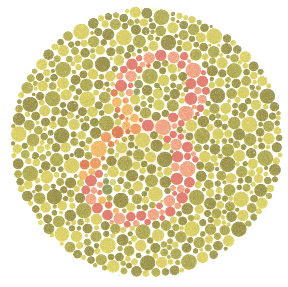
\includegraphics[width=170px]{../base/cas_4_dalton8.png}
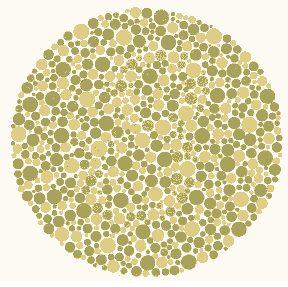
\includegraphics[width=170px]{../resultats/cas_4_dalton8_seg.png}
\end{center}
\caption{À gauche : Image initiale | À droite : Image segmentée}
\end{figure}

Nous ne pouvons pas distinguer les points formants le chiffre 8 des points formants le disque.

\subsubsection{Image {\em cas\_4\_dalton8} dans l'espace HSB}

Après conversion de l'image et segmentation, nous obtenons l'image suivante :

\begin{figure}[H]
\begin{center}
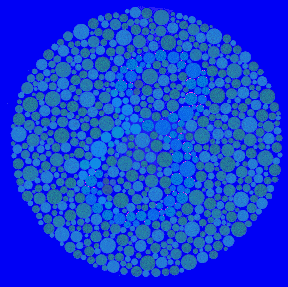
\includegraphics[width=170px]{../resultats/cas_4_dalton8_hsb.png}
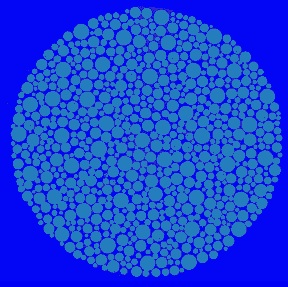
\includegraphics[width=170px]{../resultats/cas_4_dalton8_hsb_seg.png}
\end{center}
\caption{À gauche : Image initiale (HSB) | À droite : Image segmentée}
\end{figure}

Nous ne pouvons pas distinguer les points formants le chiffre 8 des points formants le disque.

\clearpage
\subsubsection{Image {\em cas\_4\_dalton29} dans l'espace RGB}

Après segmentation, nous obtenons l'image suivante :

\begin{figure}[H]
\begin{center}
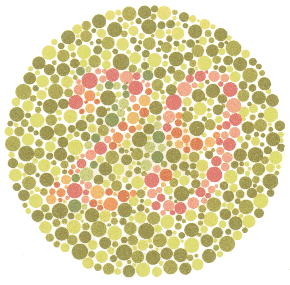
\includegraphics[width=170px]{../base/cas_4_dalton29.png}
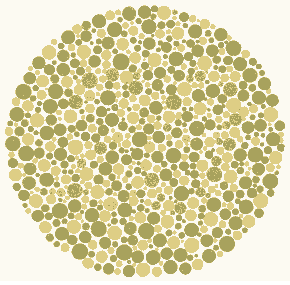
\includegraphics[width=170px]{../resultats/cas_4_dalton29_seg.png}
\end{center}
\caption{À gauche : Image initiale | À droite : Image segmentée}
\end{figure}

Nous ne pouvons pas distinguer les points formants le nombre 29 des points formants le disque.

\subsubsection{Image {\em cas\_4\_dalton29} dans l'espace HSB}

Après conversion de l'image et segmentation, nous obtenons l'image suivante :

\begin{figure}[H]
\begin{center}
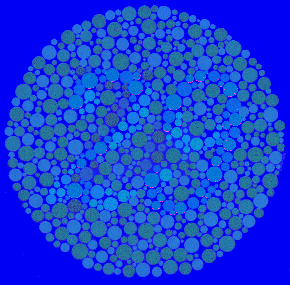
\includegraphics[width=170px]{../resultats/cas_4_dalton29_hsb.png}
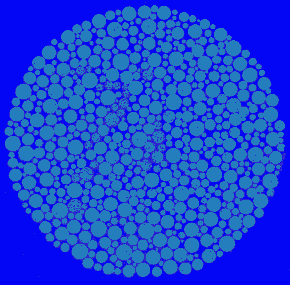
\includegraphics[width=170px]{../resultats/cas_4_dalton29_hsb_seg.png}
\end{center}
\caption{À gauche : Image initiale (HSB) | À droite : Image segmentée}
\end{figure}

Nous ne pouvons pas distinguer les points formants le nombre 29 des points formants le disque.

\clearpage
\subsubsection{Image {\em cas\_4\_dalton45} dans l'espace RGB}

Après segmentation, nous obtenons l'image suivante :

\begin{figure}[H]
\begin{center}
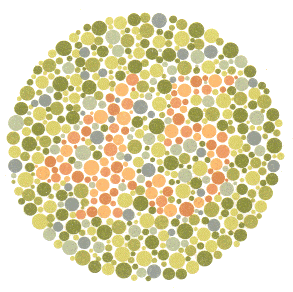
\includegraphics[width=170px]{../base/cas_4_dalton45.png}
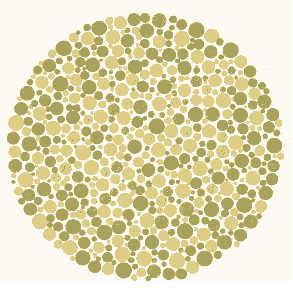
\includegraphics[width=170px]{../resultats/cas_4_dalton45_seg.png}
\end{center}
\caption{À gauche : Image initiale | À droite : Image segmentée}
\end{figure}

Nous ne pouvons pas distinguer les points formants le nombre 45 des points formants le disque.

\subsubsection{Image {\em cas\_4\_dalton45} dans l'espace HSB}

Après conversion de l'image et segmentation, nous obtenons l'image suivante :

\begin{figure}[H]
\begin{center}
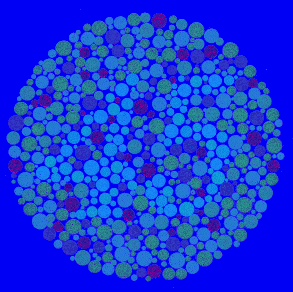
\includegraphics[width=170px]{../resultats/cas_4_dalton45_hsb.png}
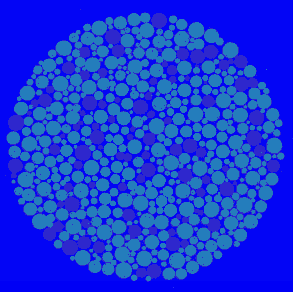
\includegraphics[width=170px]{../resultats/cas_4_dalton45_hsb_seg.png}
\end{center}
\caption{À gauche : Image initiale (HSB) | À droite : Image segmentée}
\end{figure}

Nous ne pouvons pas distinguer les points formants le nombre 45 des points formants le disque.

\clearpage
\subsubsection{Image {\em cas\_4\_dalton\_ligne} dans l'espace RGB}

Après segmentation, nous obtenons l'image suivante :

\begin{figure}[H]
\begin{center}
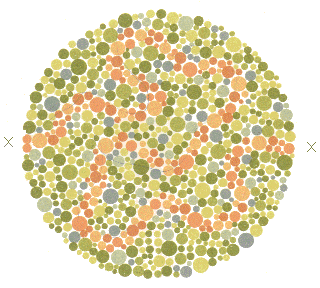
\includegraphics[width=170px]{../base/cas_4_dalton_ligne.png}
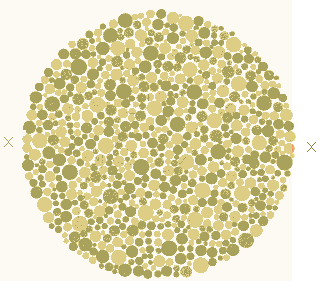
\includegraphics[width=170px]{../resultats/cas_4_dalton_ligne_seg.png}
\end{center}
\caption{À gauche : Image initiale | À droite : Image segmentée}
\end{figure}

Nous ne pouvons pas distinguer les points formants la ligne des points formants le disque.

\subsubsection{Image {\em cas\_4\_dalton\_ligne} dans l'espace HSB}

Après conversion de l'image et segmentation, nous obtenons l'image suivante :

\begin{figure}[H]
\begin{center}
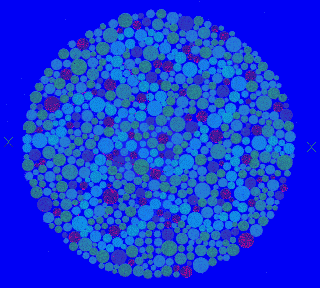
\includegraphics[width=170px]{../resultats/cas_4_dalton_ligne_hsb.png}
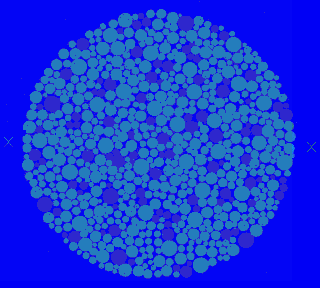
\includegraphics[width=170px]{../resultats/cas_4_dalton_ligne_hsb_seg.png}
\end{center}
\caption{À gauche : Image initiale (HSB) | À droite : Image segmentée}
\end{figure}

Nous ne pouvons pas distinguer les points formants la ligne des points formants le disque.

\clearpage
%----------------------------------------------------------------------------------------
%	CONCLUSION
%----------------------------------------------------------------------------------------

\section{Conclusion}
Après avoir défini ce qu'étaient les couleurs et leurs représentations, nous avons pu segmenter des images en un nombre donné de classes en utilisant l'algorithme K-Means Clustering.\\

Cet algorithme nous a permis -- une fois spécifié le nombre de classes voulues -- d'obtenir les couleurs de chaque classes. Une fois ces couleurs stockées, nous avons pu segmenter des images similaires en récupérant pour chaque pixel, la classe la plus proche de sa couleur.\\

Nous observons ici que les points formant les disques sont bien segmentés. Cependant, nous ne pouvons plus distinguer les nombres à l'intérieur de ces disques. Et ce aussi bien dans l'espace RGB que dans l'espace HSB.\\

Par conséquent, bien que cette méthode de segmentation soit efficace pour dissocier le fond et le disque, elle ne nous permet pas de segmenter l'image dans sa totalité.

\clearpage
%----------------------------------------------------------------------------------------

\end{document}
